Finalmente, con cada una de las partes del prototipo debidamente conectadas y calibradas y la fuente de tritio debidamente situada y asegudara, únicamente nos resta configurar la parte electŕonica del sistema para empezar a medir en el prototipo y obtener una señal adecuada. El objetivo será obtener un espectro energético de experimento con ayuda de un analizador multicanal analógico, MCA con tarjeta PCA3 y un programa Oxford WIN-MCA. 

Para ello necesitamos realizar una seríe de transformaciónes a la señal para que, por un lado,  pueda ser analizada de manera adecuada por el MCA y, por otro lado, optimicemos al máximo la señal sobre el background. El esquema electrónico utilizado se muestra en la figura 23.

\begin{figure}[hbtp]
\centering
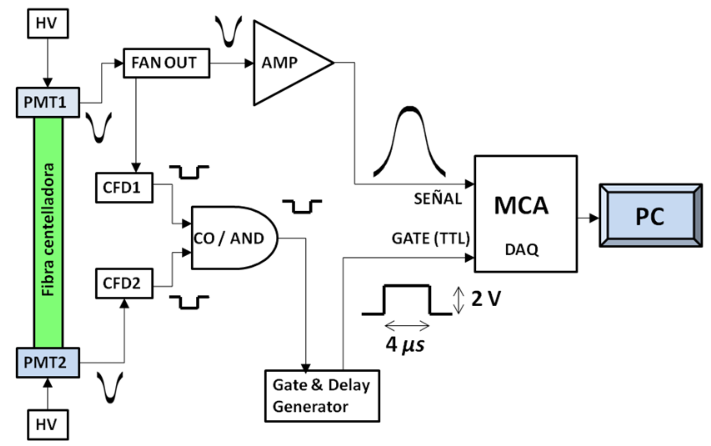
\includegraphics[scale=0.4]{Esquemaelectronico.png}
\caption{Esquema Electrico~\cite{Andres}\label{electronica}}
\end{figure}

Para conseguir cada uno de estos pasos se ha utilizado tecnología NIM. A continuación se procede a explicar el camino seguido por la señal y cada uno de los módulos que intervienen en estas transformaciones:

\begin{enumerate} 
\item{} En primer lugar sacaremos la señal de cada fotomultiplicador de la caja negra utilizada para apantallar la luz del exterior. Ello lo conseguimos con ayuda de cables BNC  ya que la caja dispone de puertos BNC macho que comunican el interior y el exterior.

\item {} Seguidamente dividimos la señales de un PMT en dos señales idénticas con ayuda de un divisor activo FAN IN/FAN OUT. Esta no es una simple división de la señal donde se produce un reparto de la intensidad sino una copia exacta de la señal de entrada. Necesitamos este típo de módulo y no una simple división ya que, como se explico al inicio del trabajo, la señal de tritio es una señal muy debil por lo que no nos podemos permitir tener pérdidas ni divisiones de esta.

\item {} Ahora dividiremos en dos caminos. Por un lado una copia de la señal del PMT que se ha duplicado, se llevará a un preamplificador (marca Tennelec) y, seguidamente, a un amplificador (marca Tennelec, modelo TC 241) con una ganancia configurada de 50. Con este camino conseguimos amplificar de manera adecuada la señal de un PMT, del orden de 60 mV hasta un total de 3V, lo cual nos permitirá optimizar el rango disponible en el MCA (Entre 0 y 5 V). Nos referiremos a la señal obtenida por este camino como señal 1.

\item{} Por otro lado, las dos señales restantes (una señal de cada PMT) serán llevada por un camino distinto para obtener una señal que nos indique cuando hay coincidencia. Para conseguir esta segunda señal hay que tener en cuenta que los PMTs ofrecen señales analógicas y negativas. Por tanto, dado que esta señal de coincidencia será creada y tratada con tecnología NIM, necesitamos convertir estas señales en señales lógicas de estándar NIM. 

Esto lo conseguimos pasando cada una de estas dos señales por un módulo discriminador (CAEN, de cuatro canales). Este ofrece una señal lógica en forma de escalón negativo de altura 1 voltio y anchura variable, en nuestro caso $30~\ns$, para cada una de las señales siempre y cuando la señal de entrada asociada supere un umbral determinado, en nuestro caso 30 mV (hablamos en valores absolutos, hay que tener en cuenta que estas son negativas). De esta forma eliminamos de manera considerable el dark current de los PMT y, por extensión, el background.

\item{} A continuación hacemos pasar ambas señales de la salida del discriminador por un módulo de conicidencias modelos Cern N 6234. Este genera una señal de salida si solo si las dos señales de entrada (procedentes de cada PMT tras pasar por el discriminador) están en coincidencia temporal. 

Estas cuatro señales (PMT, puerta lógica de cada PMT y puerta lógica de coincidencia) pueden verse en la siguiente figura:

\begin{figure}[hbtp]
\centering
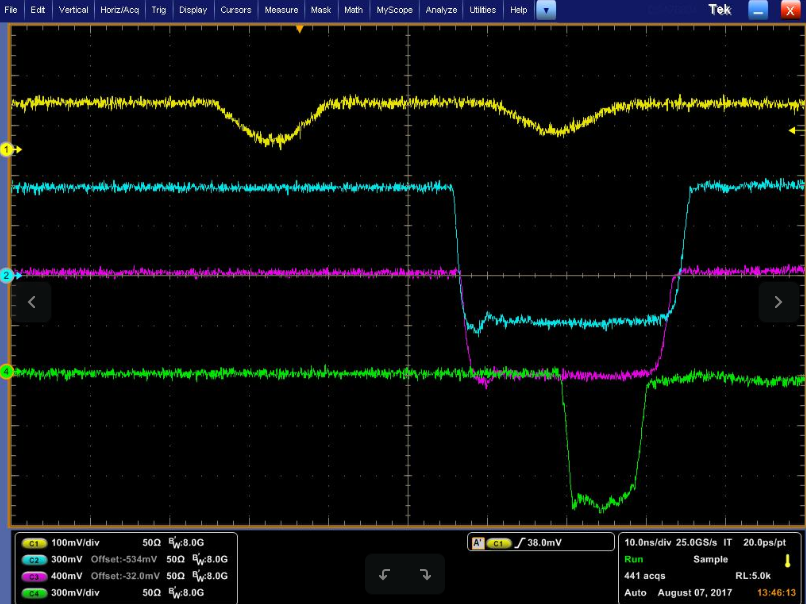
\includegraphics[scale=0.4]{SenalesNIM.png}
\caption{ Señal de salida del PMT (1), señal de salida del discriminador para cada PMT (2 y 3) y señal de salida del módulo de concidencias respectivamente\label{señales}}
\end{figure}


\item {} Luego pasamos esta señal de coincidencia a un módulo Gate \& Delay Generator (marca ORTEC, modelo 416A). Este módulo nos genera una señal lógica en forma de escalón positivo, de altura 2 voltios y anchura de $4~\mu s$, anchura suficiente para comprender en su interior la totalidad de la señal 1. Esta puerta debe ser positiva debido a que este es un requisito del MCA. Además aplicaremos un retraso a esta señal que compense la diferencia de caminos seguidos entre esta y la señal 1. Nos referiremos a la señal obtenida por este camino como señal 2.

\item {} En último lugar pasarmemos al MCA tanto la señal 1 (señal de un PMT amplificada) como la señal 2 (que nos indica cuando ambos fotomultiplicadores han detectado en coincidencia). Estas dos señales pueden verse en la siguiente figura.

\begin{figure}[hbtp]
\centering
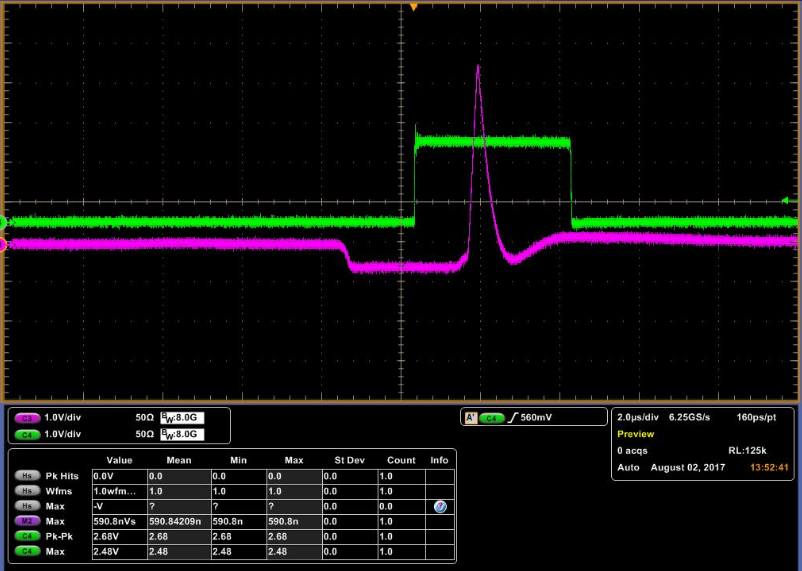
\includegraphics[scale=0.4]{SenalesMCA.png}
\caption{Señales de entrada del MCA\label{señales MCA}}
\end{figure}


Este MCA dispone de la opción de crear un histograma de señal 1 la cual solo leera mientras la señal 2 sea no nula, es decir, solo leera la señal 1 en la ventana proporcionada por la señal 2. Aquí reside la importancia de ajustar bien la anchura de la señal 2 ya que, debe de ser suficiente para contener en todo momento la señal 1 pero ajustada tanto como sea posible para evitar la entrada de dark current.

Con esto conseguimos realizar una detección en coincidencia de ambos fotomultiplicadores, lo cual nos reducirá enormemente el background del experimento.

\end{enumerate}



